
% License:
% CC BY-NC-SA 3.0 (http://creativecommons.org/licenses/by-nc-sa/3.0/)
%
%%%%%%%%%%%%%%%%%%%%%%%%%%%%%%%%%%%%%%%%%

%----------------------------------------------------------------------------------------
%	PACKAGES AND OTHER DOCUMENT CONFIGURATIONS
%----------------------------------------------------------------------------------------

\documentclass[paper=a4, fontsize=11pt]{scrartcl} % A4 paper and 11pt font size

\usepackage[T1]{fontenc} % Use 8-bit encoding that has 256 glyphs
\usepackage[utf8]{inputenc}
\usepackage{natbib}

\usepackage{fourier} % Use the Adobe Utopia font for the document - comment this line to return to the LaTeX default
\usepackage[english]{babel} % English language/hyphenation
\usepackage{amsmath,amsfonts,amsthm} % Math packages
\usepackage{lipsum} % Used for inserting dummy 'Lorem ipsum' text into the template

\usepackage{caption}
\usepackage{subcaption}
\usepackage{graphicx}

\usepackage{float}

\usepackage{blindtext} %for enumarations

\usepackage[]{hyperref}  %link collor

%talbe layout to the right
%\usepackage[labelfont=bf]{caption}
%\captionsetup[table]{labelsep=space,justification=raggedright,singlelinecheck=off}
%\captionsetup[figure]{labelsep=quad}

\usepackage{sectsty} % Allows customizing section commands
\allsectionsfont{\centering \normalfont\scshape} % Make all sections centered, the default font and small caps

\usepackage{fancyhdr} % Custom headers and footers
\pagestyle{fancyplain} % Makes all pages in the document conform to the custom headers and footers
\fancyhead{} % No page header - if you want one, create it in the same way as the footers below
\fancyfoot[L]{} % Empty left footer
\fancyfoot[C]{} % Empty center footer
\fancyfoot[R]{\thepage} % Page numbering for right footer
\renewcommand{\headrulewidth}{0pt} % Remove header underlines
\renewcommand{\footrulewidth}{0pt} % Remove footer underlines
\setlength{\headheight}{13.6pt} % Customize the height of the header

\numberwithin{equation}{section} % Number equations within sections (i.e. 1.1, 1.2, 2.1, 2.2 instead of 1, 2, 3, 4)
\numberwithin{figure}{section} % Number figures within sections (i.e. 1.1, 1.2, 2.1, 2.2 instead of 1, 2, 3, 4)
\numberwithin{table}{section} % Number tables within sections (i.e. 1.1, 1.2, 2.1, 2.2 instead of 1, 2, 3, 4)

%\setlength\parindent{0pt} % Removes all indentation from paragraphs - comment this line for an assignment with lots of text


\setlength\parskip{4pt}

%----------------------------------------------------------------------------------------
%	TITLE SECTION
%----------------------------------------------------------------------------------------

\newcommand{\horrule}[1]{\rule{\linewidth}{#1}} % Create horizontal rule command with 1 argument of height

\title{	
\normalfont \normalsize 
\textsc{IIT Roorkee} \\ [25pt] % Your university, school and/or department name(s)
\horrule{0.5pt} \\[0.4cm] % Thin top horizontal rule
\huge  Instruction Encoding for Area minimization of Instruction ROM \\ % The assignment title
\horrule{2pt} \\[0.5cm] % Thick bottom horizontal rule
}

\author{Group No. 4006\\* \\* Anuj Gupta        18114008 \\* Ankit Aharwal      18114006\\* Yashashvi Jaiswal      18114083\\* Navjit Singh      18116051\\* Nikhil Choudhary   18116054\\* Abhishek Kumar Gupta  18116001\\* Mohit Kumar      18114049\\*} % Your name

\date{\normalsize\ October 29, 2019}

\begin{document}
%\nocite{*}
\maketitle % Print the title

\newpage
\begin{abstract}

{\noindent{\Large Description} }
\\*
This topic covers the proposed instruction encoding techniques for embedded system design, which encode immediate fields of instructions , thus reduce length of overall instruction ,eventually reducing the size of an instruction memory. The comparisons between area of chips without encoding and with these encoding techniques are also made. We have to add an additional decoder for encoded values which may take some space but it is limited . When we thought of reducing the memory size, two methods came in our mind, first was decreasing the number of words but it depends on programmer and compiler.So here comes  The second method which is reducing the width of words which depends on System architecture, so we can think upon its improvement . In an instruction word, an immediate field usually determines the width (or length) of instruction words. However, there is no existing application that all values which can be represented by the immediate field are used. In this project, we try to implement instruction encoding techniques, which encode immediate fields of instructions to reduce the size of the instruction memory.
  \\


\textbf{Key words:} encoding, decoding ,computer architecture, immediate
\end{abstract}

\begin{abstract}

{\noindent{\Large \\*  Why this Topic is Important} }
\\*
Small memory size for instruction encoding means better use chip size. Smaller chips have much more advantage than bigger chips. 
\begin{itemize}
\item They are small hence less material is required and cost price is reduced. 
\end{itemize}
\begin{itemize}
\item They consume very less power. 
\end{itemize}
\begin{itemize}
\item They can be cooled easily because they work on less power. 
\end{itemize}
\\* One may argue according to Stefan-Boltzmann law that surface area (A)  heat  is proportional to heat transfer per unit time (q). But in case of chips heat generated by them is bigger factor than heat transfer rate.
This topic also interesting because as we know Moore law is ending,as we can no longer make chips small by doubling number of transistors on a microchip doubles about every two years. To achieve more smaller chips we have to find new and innovative solutions.
  \\

\end{abstract}

\begin{abstract}

{\noindent{\Large \\* Methods used for Evaluation and Discussion} }\\
   
    In this paper , there are 6 different types of encoding techniques to encode the immediate value. With the help of these techniques in different situations we can reduce the memory, thus area of chip.\\* \\* \\*
    \begin{figure}[h!]
\centering
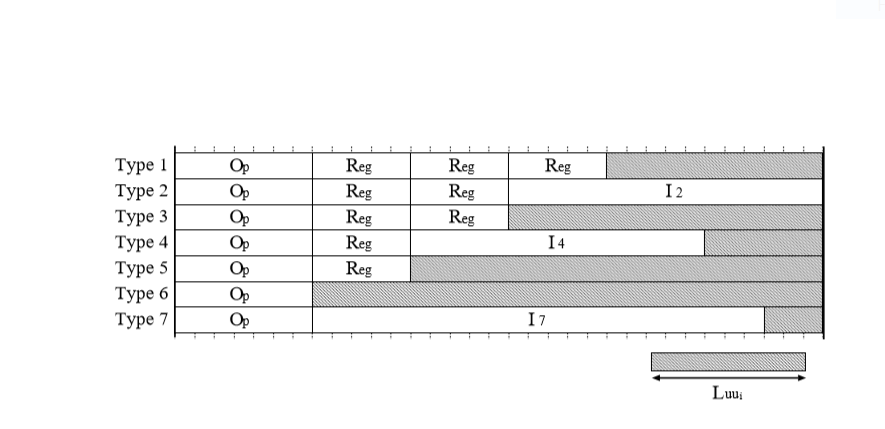
\includegraphics[scale=1]{instruction.jpg}
\caption{DIfferent types of instructions.}
\label{fig:instruction}
\end{figure}
\\*
    There are 7 different types of instructions. Each type of instruction has operation code, and their may be registers or immemdiate vaues or both.\\*
    However we are intrested only in Type 2, Type 4 and Type 7 instructions because they only contain immediate values.\\*
    Basically what we are doing in all these 6 techniques are while encoding the instruction , it calls the WRITE module and the no. is written or stored in a separate file one by one . And in instruction we will use e.g. ADD L1,L1,00 instead of ADD L1,L1,34 . So we are using encoded version. In this example , while accesing 00 it will call READ module and will pick up the original no. to which this encoded no. is mapped. So our ROM area is reduced.
    \\* Here are our 6 encoding techniques for reducing max of length of instructions.
    \\*\\*
    1. Longest / All Coding(LAC)\\*
    This is the most basic and fundamental instruction encoding technique.
    LAC is a method to encode only the immediate values of the longest instruction format type which is Type 2. We insert all Type 2 instructions in memory. where its index is saved in place of immediate value in the ROM.
    In this figure, the shaded part is the immediate field eliminated by encoding. Figure 5 contains LAC.
    \\*\\*
    2. Individual format/All Coding (IAC)\\*
    IAC is a method to encode the immediate values of each field of type 2, type 4, and type 7 individually.Hence, we have to save immediate values at three different memory locations. This is also slightly complex due this. Figure 6 shows IAC.\\*\\*
    
\begin{figure}[h!]
\centering
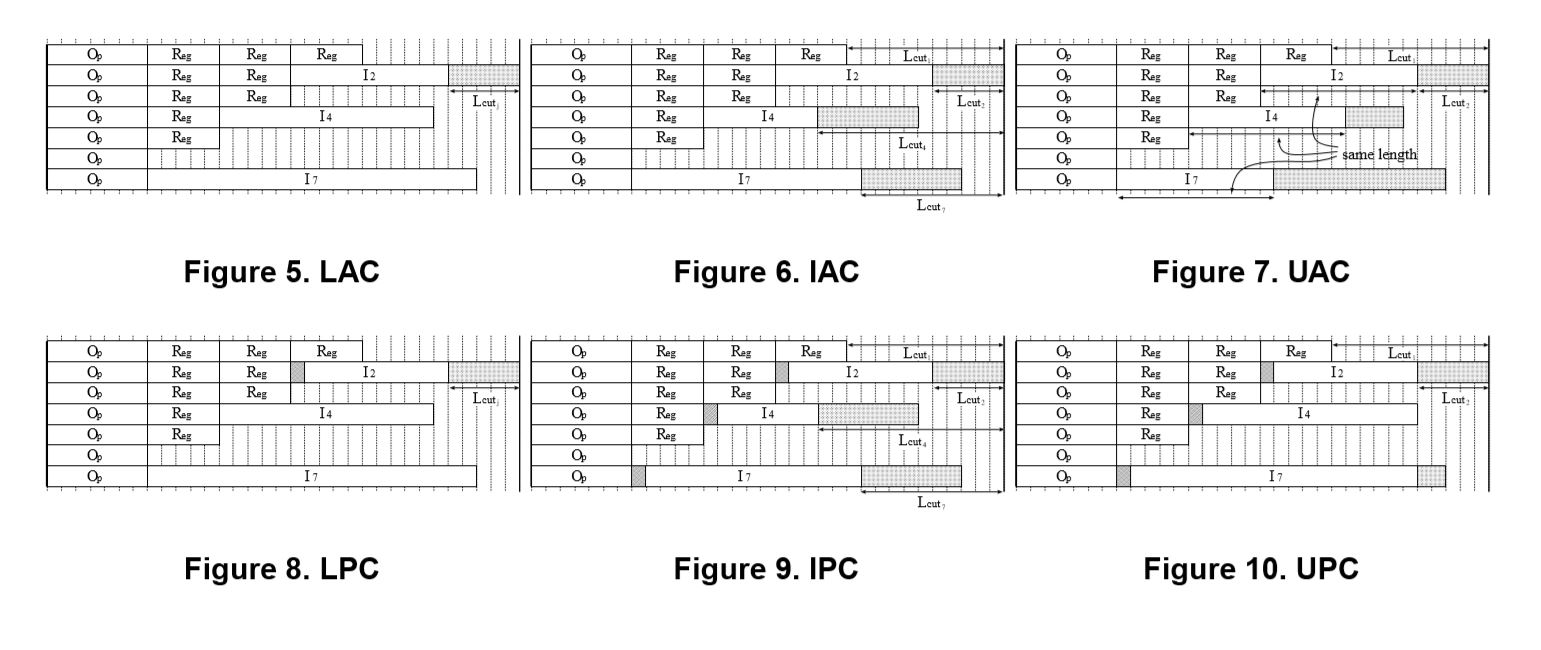
\includegraphics[scale=0.6]{figure.jpg}
\caption{Types of instruction encodings}
\label{fig:instruction encodings}
\end{figure}

    3.Union format/All Coding (UAC)\\*
    UAC is a method to encode the immediate values of each field of type 2, type 4, and type 7 altogether.Hence the memory used for storing is greatest and also its the most compressing in nature among IAC and LAC. Figure 7 shows UAC.\\*\\*
    4. LONGEST/PARTIAL CODING(LPC)
    \\*LPC is almost same as LAC the only difference in being it first compares the whether its actually effiecient to encode the value or not.
    LPC encodes only the immediate values of the longest instruction format type. It does not encode the values which can be represented in an immediate field after encoding. e.g. if 0 and 1000 are the immediate value, 0 need not be encoded, 1000 will be encoded as 1. The purpose of this method is to reduce the size of the immediate decoder. In this case, a flag bit to indicate whether the values is encoded or not is necessary. The hatched part is the flag bit. Figure 8 contains LPC.
    \\*\\*
    5. INDIVIDUAL/PARTIAL CODING(IPC)\\*
    IPC is very similiar to IAC except it also first compares whether its more efficient to encode value or not.IPC is a method to encode the immediate values of each field of type 2, type 4, and type 7 individually. Suppose we are having immediate value bits less than the number of encoded data index bits than it will not encode that particular value. However due to this we have to add an extra flag digit which in this particular case would be 0.Figure 9 contains IPC.
    \\*\\*
    6. UNION/PARTIAL CODING (UPC)\\*
    UPC is a method to encode the immediate values of each field of type 2, type 4, and type 7 altogether. Similar to LPC, it does not encode the values which can be represented in an immediate field after encoding, and the flag bit is necessary. Figure 10 shows UPC. Because the number of encoded immediate values changes depending on the size of the fields I2, I4, and I7, we think about size by arranging a right edge of an immediate field as shown in Figure 10. field I4 is Lreg bits longer than field I2, and fieldI7 is 2*Lreg bits longer than field I2. 
    \\*\\*
    

    
 
\end{abstract}
\begin{abstract}

{\noindent{\Large \\* \\* \\*Results and Conclusion} }
\\* \\*While implementing this idea, the main motive was to reduce the size of instruction and we have achieved reduction in instruction size in all these techniques whether it be LAC, IAC, UAC, LPC, IPC, UPC with more or less same applicability.\\*
LAC, IAC, UAC being more simple and fast.\\*IAC performed very better in compare to LAC and UAC.\\*LPC, IPC and UPC being more complex, efficient and little slower.
Those three almost performed equally in all tests.\\*
UAC was the most underperforming among all 6 techniques.\\*
We have exhausted the ability of maximizing the reduction ratio of ROM area which even include decoder for immediate values.\\*
As we can see if the proposed techniques are applied to real data of instruction sets, the dramatic boost in cost reduction will be visible to us.\\*\\*
\end{abstract}

\citep{main_paper}
\citep{second_paper}
\citep{third_paper}
\bibliography{references}

\bibliographystyle{plain}
\end{document}